\chapter{Capa de Negocio}
\section{Introducción}
contenido...
\newpage
\section{Punto de Vista de Organización}
\subsection{Modelo}
El punto de vista de la Organización se centra en la organización (interna) de una empresa, un departamento, una red de empresas u otra entidad organizativa. Es posible presentar los modelos en este punto de vista como diagramas de bloques anidados, pero también de una manera más tradicional, como gráficos de la organización. El punto de vista de la Organización es muy útil para identificar competencias, autoridades y responsabilidades.\\

\begin{figure}[h!]
	\centering
	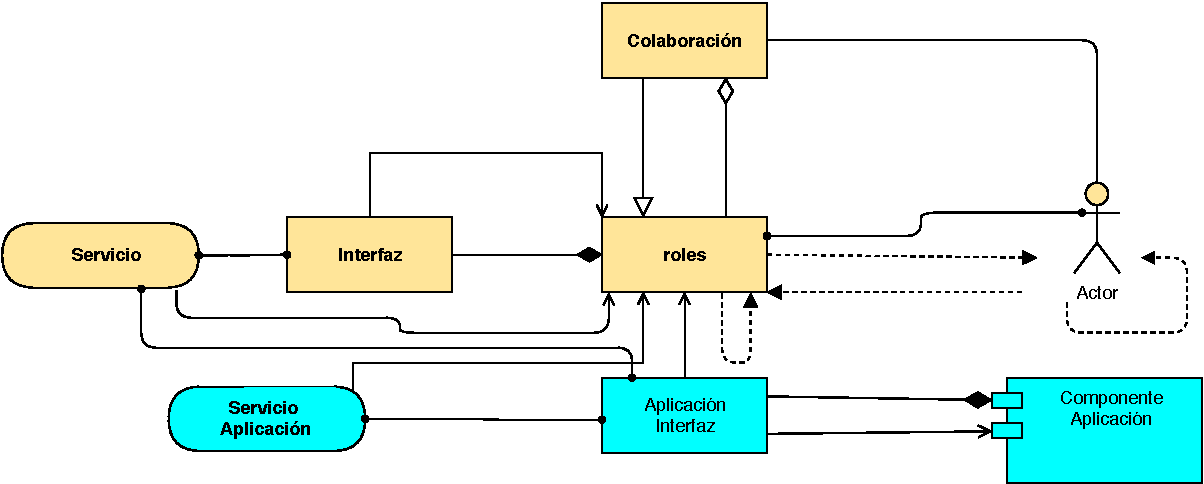
\includegraphics[width=1\linewidth]{ARQUITECTURA/imgs/MOrganizacion}
	\caption{Modelo de Ogranización}
\end{figure}


\newpage
\subsection{Caso de Estudio}

\begin{figure}[h!]
	\centering
	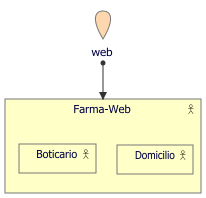
\includegraphics[width=.5\linewidth]{ARQUITECTURA/imgs/COrganizacion}
	\caption{Modelo de Ogranización}
\end{figure}

 Explicacmos nuestro caso de estudio
\newpage
%---------------------------------
\section{Punto de Vista de Coperación de Actor}
\subsection{Modelo}
El punto de vista de la cooperación del actor se centra en las relaciones de los actores entre sí y su entorno. Un ejemplo común de esto es el "diagrama de contexto", que pone una organización en su entorno, que consiste en partes externas como clientes, proveedores y otros socios comerciales. Es muy útil para determinar dependencias externas y colaboraciones. Muestra la cadena o red de valor en la que opera el actor.\\\\
 
Otro uso importante del punto de vista de la cooperación del actor es mostrar cómo los actores operativos del negocio y / o los componentes de la aplicación juntos realizan un proceso comercial.
\\\\
Por lo tanto, desde este punto de vista, pueden ocurrir tanto actores o roles empresariales como componentes de aplicaciones.

\begin{figure}[h!]
	\centering
	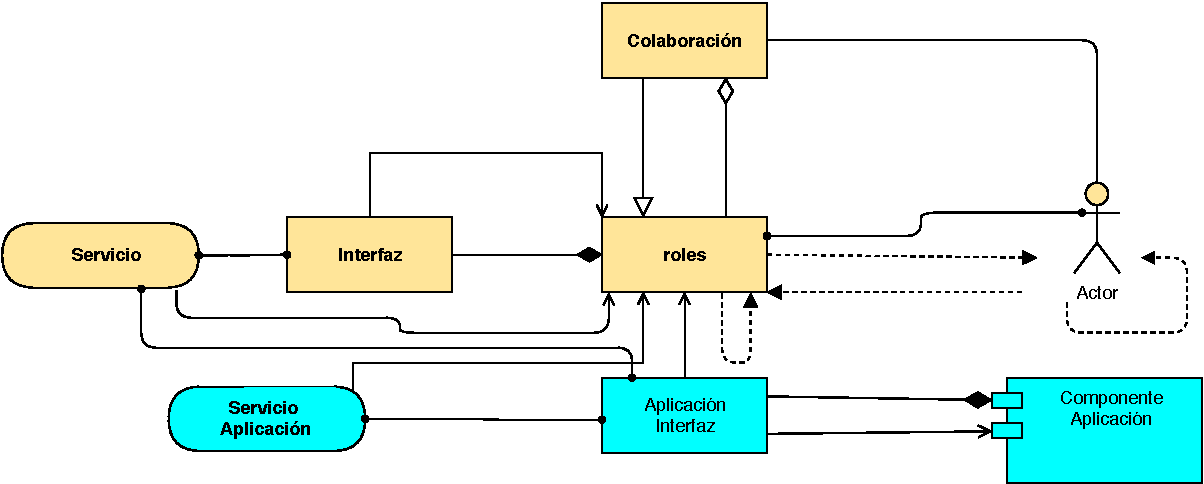
\includegraphics[width=1\linewidth]{ARQUITECTURA/imgs/MOrganizacion}
	\caption{Modelo de Ogranización}
\end{figure}


\newpage
\subsection{Caso de Estudio}

\begin{figure}[h!]
	\centering
	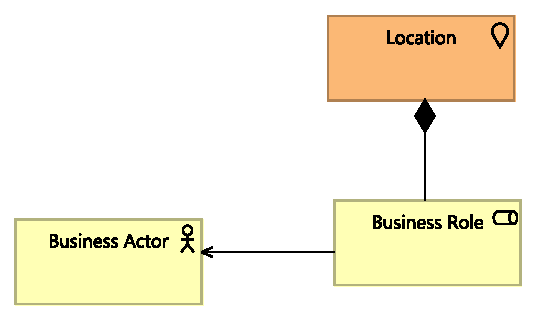
\includegraphics[width=.5\linewidth]{ARQUITECTURA/imgs/COrganizacion1}
	\caption{Modelo de Ogranización}
\end{figure}
Explicacmos nuestro caso de estudio
\newpage
%---------------------------------
\section{Punto de Vista de Fcunión de Negocio}
\subsection{Modelo}
The Organization viewpoint focuses on the (internal) organization of a company, a department, a network of companies, or of another organizational entity. It is possible to present models in this viewpoint as nested block diagrams, but also in a more traditional way, such as organizational charts. The Organization viewpoint is very useful in identifying competencies, authority, and responsibilities in an

\begin{figure}[h!]
	\centering
	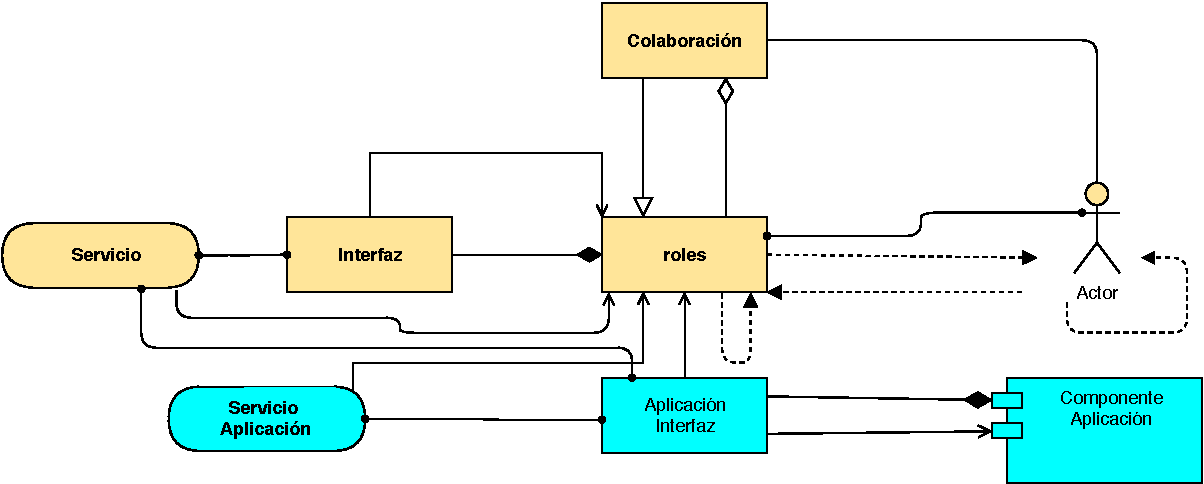
\includegraphics[width=1\linewidth]{ARQUITECTURA/imgs/MOrganizacion}
	\caption{Modelo de Ogranización}
\end{figure}


\newpage
\subsection{Caso de Estudio}

\begin{figure}[h!]
	\centering
	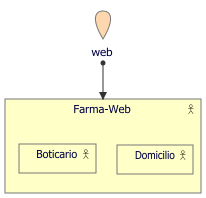
\includegraphics[width=.5\linewidth]{ARQUITECTURA/imgs/COrganizacion}
	\caption{Modelo de Ogranización}
\end{figure}
Explicacmos nuestro caso de estudio
\newpage
%---------------------------------
\section{Punto de Vista de Proceso de Negocio}
\subsection{Modelo}
The Organization viewpoint focuses on the (internal) organization of a company, a department, a network of companies, or of another organizational entity. It is possible to present models in this viewpoint as nested block diagrams, but also in a more traditional way, such as organizational charts. The Organization viewpoint is very useful in identifying competencies, authority, and responsibilities in an

\begin{figure}[h!]
	\centering
	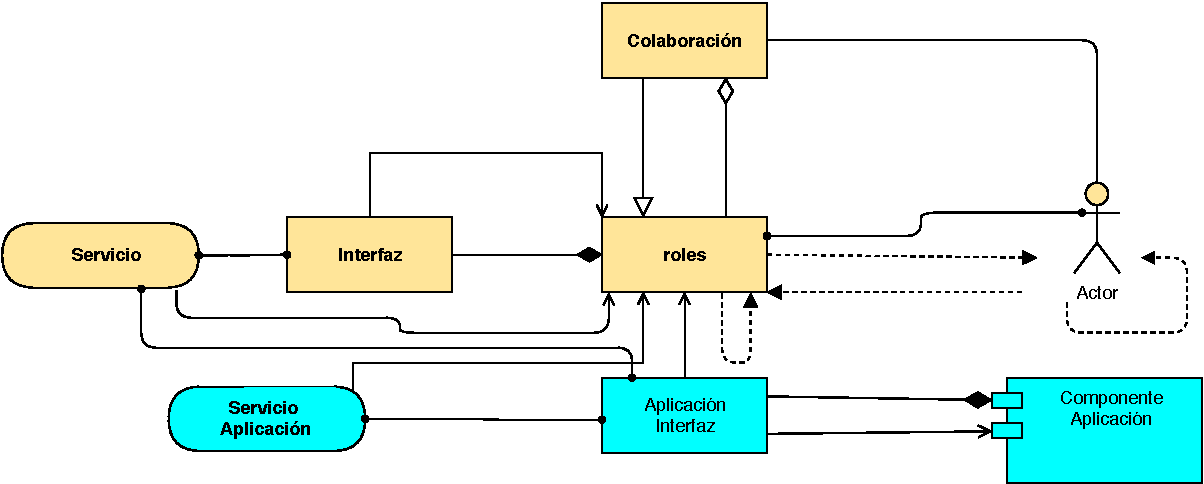
\includegraphics[width=1\linewidth]{ARQUITECTURA/imgs/MOrganizacion}
	\caption{Modelo de Ogranización}
\end{figure}


\newpage
\subsection{Caso de Estudio}

\begin{figure}[h!]
	\centering
	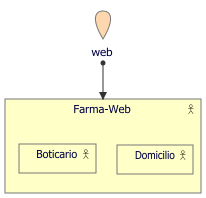
\includegraphics[width=.5\linewidth]{ARQUITECTURA/imgs/COrganizacion}
	\caption{Modelo de Ogranización}
\end{figure}
Explicacmos nuestro caso de estudio
\newpage
%---------------------------------
\section{Punto de Vista de Cooperación de Proceso de Negocio}
\subsection{Modelo}
The Organization viewpoint focuses on the (internal) organization of a company, a department, a network of companies, or of another organizational entity. It is possible to present models in this viewpoint as nested block diagrams, but also in a more traditional way, such as organizational charts. The Organization viewpoint is very useful in identifying competencies, authority, and responsibilities in an

\begin{figure}[h!]
	\centering
	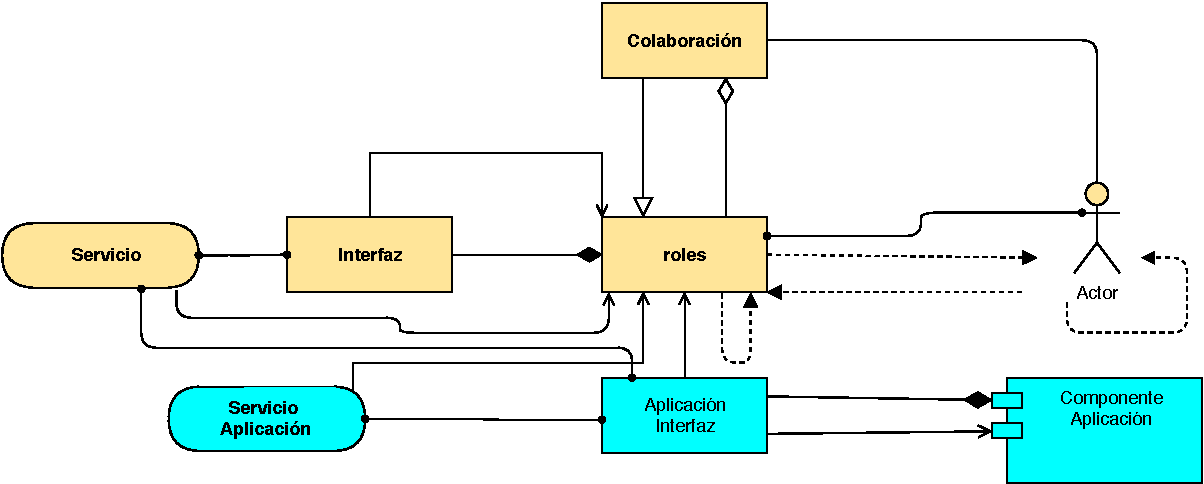
\includegraphics[width=1\linewidth]{ARQUITECTURA/imgs/MOrganizacion}
	\caption{Modelo de Ogranización}
\end{figure}


\newpage
\subsection{Caso de Estudio}

\begin{figure}[h!]
	\centering
	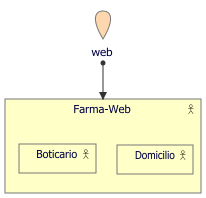
\includegraphics[width=.5\linewidth]{ARQUITECTURA/imgs/COrganizacion}
	\caption{Modelo de Ogranización}
\end{figure}
Explicacmos nuestro caso de estudio
\newpage

%---------------------------------
\section{Punto de Producto}
\subsection{Modelo}
The Organization viewpoint focuses on the (internal) organization of a company, a department, a network of companies, or of another organizational entity. It is possible to present models in this viewpoint as nested block diagrams, but also in a more traditional way, such as organizational charts. The Organization viewpoint is very useful in identifying competencies, authority, and responsibilities in an

\begin{figure}[h!]
	\centering
	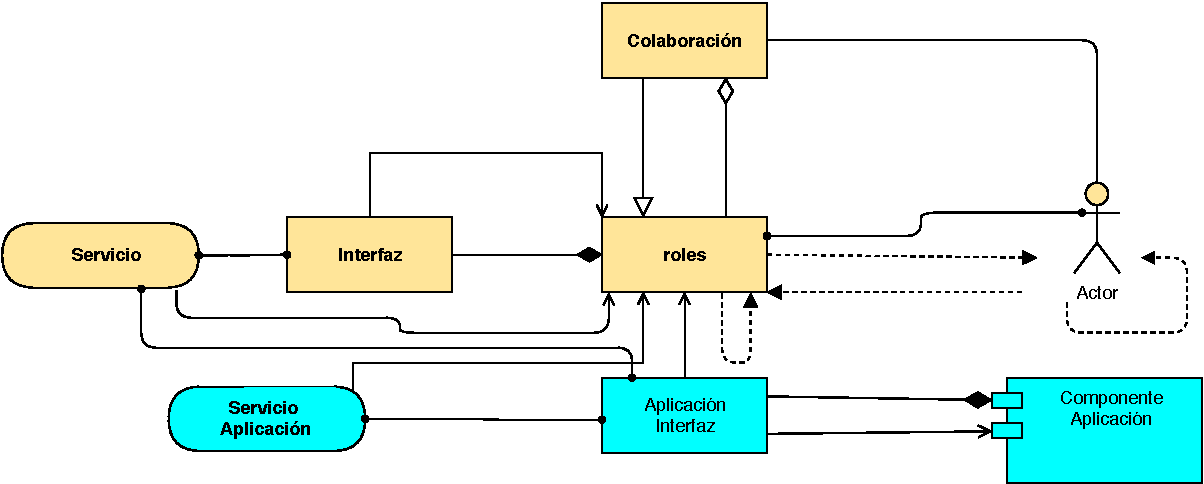
\includegraphics[width=1\linewidth]{ARQUITECTURA/imgs/MOrganizacion}
	\caption{Modelo de Ogranización}
\end{figure}


\newpage
\subsection{Caso de Estudio}

\begin{figure}[h!]
	\centering
	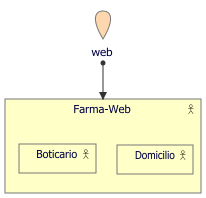
\includegraphics[width=.5\linewidth]{ARQUITECTURA/imgs/COrganizacion}
	\caption{Modelo de Ogranización}
\end{figure}
Explicacmos nuestro caso de estudio
\newpage
